In this section we will discuss the different methods required to effectively run classical computational simulations of the protocols described in Section \ref{section:protocols} such that, for any choice of qubit pure states and rank-1 POVMs, the quantum predictions in Equation (\ref{eq:prob_quantum}) are reproduced classically following Equation (\ref{eq:prob_classic}), i.e.
\begin{equation}
\forall \rho, \{B_b\}:\quad tr(\rho B_b) = \int_{\lambda} d\lambda\ \pi(\lambda) \sum_{c=1}^{d_C} p_A(c|\rho, \lambda) p_B(b|\{B_b\}, c, \lambda)    
\end{equation}

The main goal is to carry out these simulations using standard classical computations, but some particular results will be confronted with the outcomes from quantum circuit simulators, therefore there will be specific subsections devoted to the implementation of generalized measurements in a quantum circuit model. 
\subsection{State preparation}
In the classical simulations, the state preparation would require to produce a random qubit pure state first, and then to compute the corresponding Bloch vector to be later used by Alice. 

In the prepare-and-measure scenario, Alice uses the Bloch vector representation of the qubit's pure state, and Bob's POVMs,  proportional to rank-1 projectors, are expressed as the outer product of the associated Bloch vectors. In the Bell scenario, Alice also uses the Bloch vector corresponding to the local projective measurement projectors. Given the fact that the classical and quantum probabilities must be equivalent for any state and POVM set, it is therefore of key importance to be able prepare random Bloch vectors uniformly distributed along the unit radius sphere $S_2$. In addition, in all these simulation protocols, Alice and Bob share two normalized vectors $\vec{\lambda}_1, \vec{\lambda}_2 \in \mathbb{R}^{3}$, which must be uniformly and independently distributed on the same unit sphere $S_2$. Hence the randomized Bloch vector preparation is not only the building block for the state preparation, but also plays a critical role in the measurement construction and shared randomness creation.

To produce a random qubit pure state, we should obtain a random unitary matrix and then apply the unitary transformation to the zero qubit state, resembling the time evolution of a qubit from a zero initial state. The random unitary matrix can be generated by just building a matrix of normally distributed complex numbers, and then apply the Gram-Schmidt QR decomposition to orthogonalize the matrix, see \cite{ozols2009}, \cite{zyczkowski1994}. 

The resulting random qubit state distribution could be validated using the corresponding Bloch vector distribution along the unit radius sphere. A tessellation scheme called HEALPix \cite{healpix}, which produces a hierarchical and equal-area iso-latitude pixelation of a sphere, could be used to show that the random Bloch vectors are uniformly and independently distributed in the Bloch sphere. Given that each pixel in HEALPix covers the same surface area as every other pixel (see Figure \ref{fig:healpix_sphere}), we could group the Bloch vector distribution along the different pixel indices (see Figure \ref{fig:healpix_numbering}), and check whether the resulting distribution is uniform as expected.

\begin{figure}[!ht]
\begin{center}
\centerline{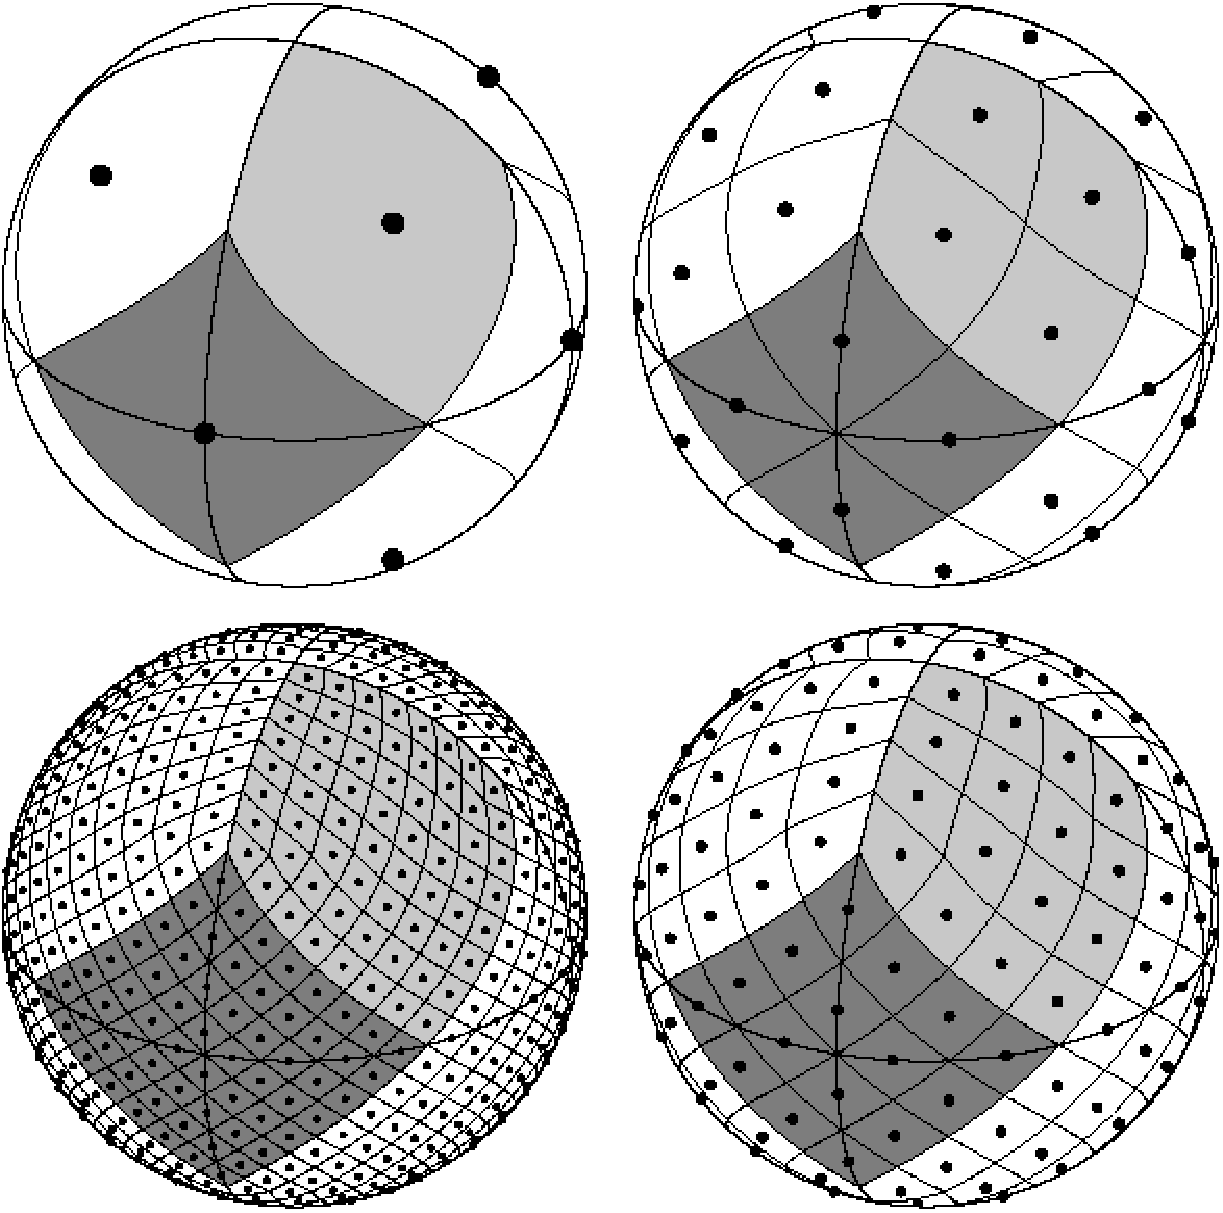
\includegraphics[height=5.5cm]{images/healpix4.pdf}}
\caption[Orthographic view of Healpix partition of the sphere]%
{\label{fig:healpix_sphere}%
Orthographic view of HEALPix partition of the sphere.}
\end{center}
\end{figure}

\begin{figure} [!ht]
\begin{center}
\centerline{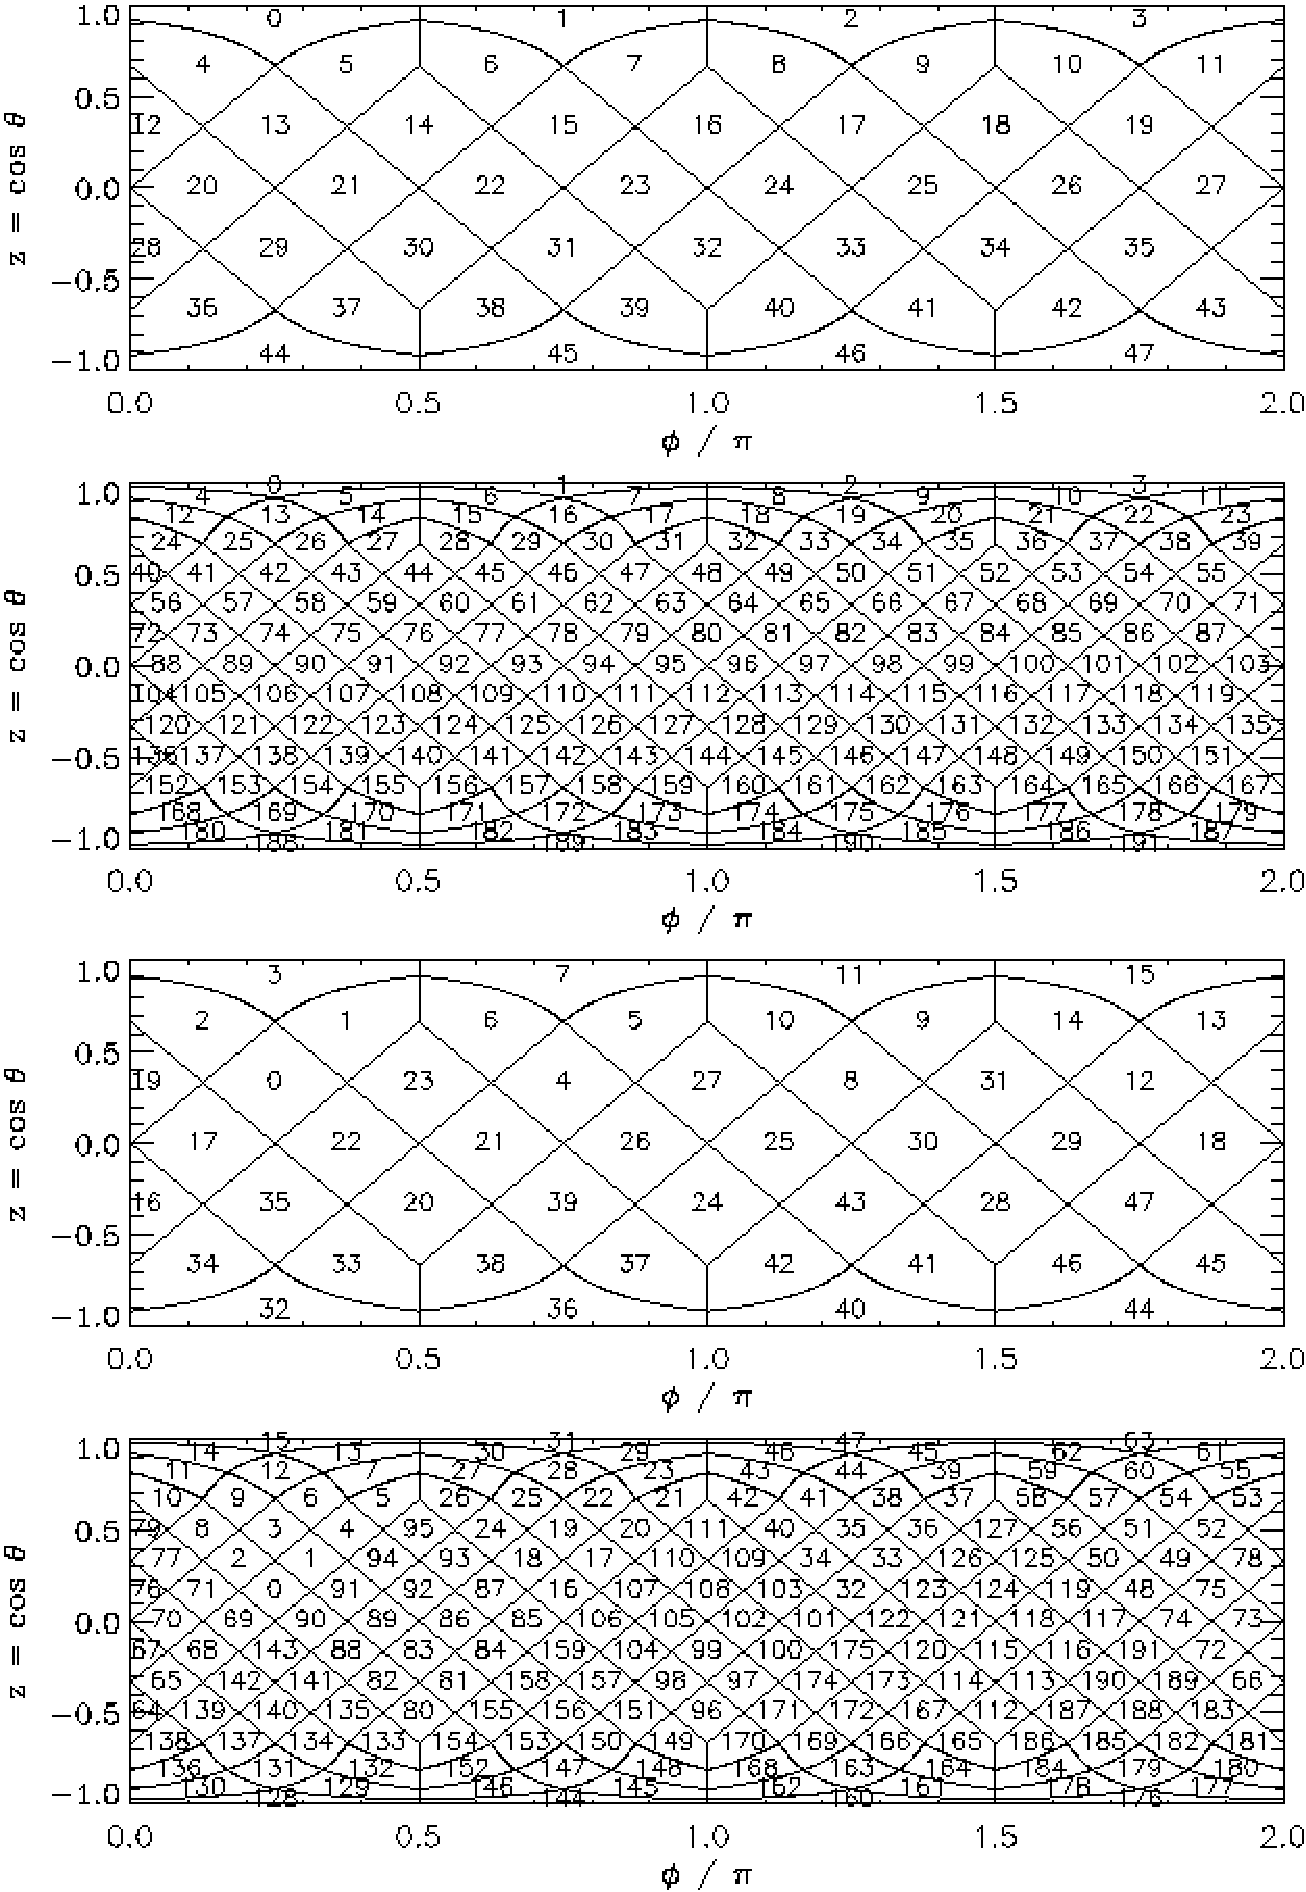
\includegraphics[height=10.5cm]{images/healpix2d.pdf}}
\caption[Cylindrical projection]%
{\label{fig:healpix_numbering}%
Cylindrical projection of the HEALPix division of a
sphere and two natural pixel numbering schemes (RING and NESTED). 
Both numbering schemes map the two dimensional 
distribution
of discrete area elements on a sphere into the one dimensional, 
integer pixel number array.
}
\end{center}
\end{figure}
\subsection{Rank-1 POVMs implementation}
We have already discussed how every qubit POVM can be written as a coarse graining of rank-1 projectors \cite{barrett2002}, such that the protocol implementation can restrict without any loss in generality to POVMs proportional to rank-1 projectors. 

Even if the final goal is to build POVMs to test how the classical protocol converges with the quantum theory for any random state and measurement, we will also discuss some general rank-1 POVMs with interesting properties, for example, 
\begin{enumerate}
    \item The measure needed in the eavesdropping  of the BB84 protocol \cite{nielsen2000}
\begin{equation}
    \mathbb{P}_4 = \{\frac{1}{2}\ket{0}\bra{0}, \frac{1}{2}\ket{1}\bra{1}, \frac{1}{2}\ket{+}\bra{+}, \frac{1}{2}\ket{-}\bra{-} \}
\end{equation}
    \item The Trine-POVM, consisting of POVM elements uniformly distributed on an equatorial plane of the Bloch sphere
\begin{equation}
\{\ket{\Psi_1}=\ket{0},\ \ket{\Psi_2}=\frac{1}{2}\ket{0} + \frac{\sqrt{3}}{2} \ket{1},\ \ket{\Psi_3}=\frac{1}{2}\ket{0} - \frac{\sqrt{3}}{2} \ket{1}\}
\end{equation}
    \item The SIC-POVMs, a well-known family of symmetric informationally complete positive operator-valued measures, which are proven to be very relevant in quantum state tomography and quantum cryptography fields among others \cite{renes2004}. The simplest SIC-POVM is the one with states the vertices of a regular tetrahedron in the Bloch sphere, see Figure \ref{fig:sic_povm}.
\end{enumerate}

The strategies to build the rank-1 POVMs and perform the measurement are different in the classical simulation protocol and in the quantum circuit model, as we will see later, so next sections will go through the methodologies applied for each case.

\begin{figure}[!ht]
\begin{center}
\centerline{\includesvg[height=4cm]{images/sic_povm.svg}}
\caption[SIC-POVM as tetrahedron in Bloch sphere]%
{\label{fig:sic_povm}%
In the Bloch sphere representation of a qubit, the states of a SIC-POVM form a regular tetrahedron with vertices $\ket{\Psi_1}=\ket{0}$, $\ket{\Psi_2}=1/{\sqrt{3}}\ket{0} + \sqrt{2/3} \ket{1}$, $\ket{\Psi_3}=1/{\sqrt{3}}\ket{0} + \sqrt{2/3} \ e^{i\frac{2\pi}{3}} \ket{1}$ and $\ket{\Psi_4}=1/{\sqrt{3}}\ket{0} + \sqrt{2/3}\ e^{i\frac{4\pi}{3}} \ket{1}$.}
\end{center}
\end{figure}

\subsubsection{Measurement in classical simulation protocols}
As described by Sent\'is et al.\ \cite{sentis2013}, the conditions under which a set of $N$ arbitrary rank-1 operators $\{E_{k}\}$ comprises a qubit POVM such that $\sum_{k=1}^{N} a_{k} E_{k} = \mathbb{1}$, can be equivalently written in a system of four linear equations
\begin{equation}
    \sum_{k=1}^{N} a_{k} = 2
\end{equation}
\begin{equation}
    \sum_{k=1}^{N} a_{k} \vec{y}_{k} = \vec{0}
\end{equation}
where $\vec{y}_{k} \in \mathbb{R}^3$ are the Bloch vectors corresponding to the qubit pure states $\ket{v_{k}}$. The existence of the set $\{a_{k}\}$ has a direct translation into a linear programming feasibility problem we would have to solve computationally.

As an example, to build a random POVM set of $N=4$ elements, we could apply the following procedure:
\begin{enumerate}
\item Assign two rank-1 operators as projective measurement elements $E_i = \ket{v_i}\bra{v_i}$ with unknown weights $\{a_i\} \text{, where}\ i=1,2$.
\item Apply the closure relation such that the third rank-1 operator is $E_3 = \mathbb{1} - \sum_{i=1}^{2}E_i$. Note that this will not be necessarily a rank-1 operator.
\item Diagonalize $E_3$ to obtain the relevant qubit states as eigenvectors $\ket{v_3}$ and $\ket{v_4}$.
\item Convert all quibit states $\ket{v_i}$ to Bloch vectors $\vec{y}_i \text{, where } i=1,2,...4$.
\item Solve the linear programming feasibility problem
\begin{equation*}
\begin{array}{ll@{}ll}
\textbf{find}  & x = \{a_1, a_2,\dots,a_N\} &\\
\textbf{subject to}& Ax = b\ \text{where column} \ A_{*k} = (\vec{y}_k, 1),\ \text{and}\ b = (\vec{0}, 2) \\
                 & x \geq 0 
\end{array}
\end{equation*}
\end{enumerate}

Provided the optimization problem is feasible, we obtain the weights $\{a_k\}$ and compute the rank-1 operators $\{E_k\}$ conforming the POVM set elements $B_k=a_k E_k$. Then we can use Equation \ref{eq:rank1_povm} to perform the following assignment
\begin{equation}
    p_k = \frac{a_k}{2}
\end{equation}
\begin{equation}
    \ket{\vec{y}_k}\bra{\vec{y}_k} = E_k
\end{equation}
which will implement the POVMs in the form required by the classical simulation protocols, i.e. $B_{k} = 2p_{k}\ket{\vec{y}_{k}}\bra{\vec{y}_{k}}$.

\subsubsection{Measurement in quantum circuit model}
One of the objectives of this project is to compare the probability distributions obtained with the classical simulation protocols, against the distributions derived when performing generalized measurements on either quantum simulators or noisy intermediate-scale quantum computers. For the sake of such comparison, we must devise a method to encode positive operator-valued measures in a quantum circuit model.
Peres \cite{peres1995}

\begin{equation}
B_{k} = \ket{v_{k}} \bra{v_{k}}
\end{equation}

\begin{equation}
\ket{w_{k}} := \ket{v_{k}} + \sum_{s=d_{Q}+1}^{N} c_{k s} \ket{u_{k}}
\end{equation}

\begin{equation}
\bra{w_{j}} \ket{w_{k}} := \bra{v_{j}} \ket{v_{k}} + \sum_{s=d_{Q}+1}^{N} c_{j s}^{\star} c_{k s} = \delta_{j k}
\end{equation}

\begin{equation}
\sum_{i=1}^{n} v_{j i}^{\star} v_{k i} + \sum_{s=d_{Q}+1}^{N} c_{j s}^{\star} c_{k s} = \delta_{j k}
\end{equation}

\begin{equation}
\sum_{k=1}^{N}\ket{v_{k}}\bra{v_{k}} = \sum_{k=1}^{N} B_{k} = \mathbb{1}
\end{equation}


\begin{equation}
\sum_{k=1}^{N}v_{k i}^{\star} v_{k j} = \delta_{ij}
\end{equation}

\begin{equation}
M = 
\begin{pmatrix}
v_{1 1} & \dots & v_{1 d_{Q}} & c_{1,d_{Q}+1} & \dots & c_{1 N} \\
v_{2 1} & \dots & v_{2 d_{Q}} & c_{2,d_{Q}+1} & \dots & c_{2 N} \\
\vdots &  & \vdots & \vdots &  & \vdots \\
v_{N1} & \dots & v_{Nd_{Q}} & c_{N,d_Q+1} & \dots & c_{NN}
\end{pmatrix}    
\end{equation}

\[\mathcal{H}^{d_Q}\ \mathcal{K}^{N}\]
\subsection{Prepare-and-measure simulations}
\subsubsection{Classical transmission of one qubit}
\textit{TBW}
\subsubsection{Quantum circuit counterpart}
Peres \cite{peres1995}

\begin{equation}
B_{\mu} = \ket{v_{\mu}} \bra{v_{\mu}}
\end{equation}

\begin{equation}
\ket{w_{\mu}} := \ket{v_{\mu}} + \sum_{s=d_{Q}+1}^{N} c_{\mu s} \ket{u_{\mu}}
\end{equation}

\begin{equation}
\bra{w_{\lambda}} \ket{w_{\mu}} := \bra{v_{\lambda}} \ket{v_{\mu}} + \sum_{s=d_{Q}+1}^{N} c_{\lambda s}^{\star} c_{\mu s} = \delta_{\lambda \mu}
\end{equation}

\begin{equation}
\sum_{i=1}^{n} v_{\lambda i}^{\star} v_{\mu i} + \sum_{s=d_{Q}+1}^{N} c_{\lambda s}^{\star} c_{\mu s} = \delta_{\lambda \mu}
\end{equation}

\begin{equation}
\sum_{\mu=1}^{N}\ket{v_{\mu}}\bra{v_{\mu}} = \sum_{\mu=1}^{N} B_{b,\mu} = \mathbb{1}
\end{equation}


\begin{equation}
\sum_{\mu=1}^{N}v_{\mu i}^{\star} v_{\mu j} = \delta_{ij}
\end{equation}

\begin{equation}
M = 
\begin{pmatrix}
v_{\alpha 1} & \dots & v_{\alpha d_{Q}} & c_{\alpha,d_{Q}+1} & \dots & c_{\alpha N} \\
v_{\beta 1} & \dots & v_{\beta d_{Q}} & c_{\beta,d_{Q}+1} & \dots & c_{\beta N} \\
\vdots &  & \vdots & \vdots &  & \vdots \\
v_{N1} & \dots & v_{Nd_{Q}} & c_{N,d_Q+1} & \dots & c_{NN}
\end{pmatrix}    
\end{equation}

\[\mathcal{H}^{d_Q}\ \mathcal{K}^{N}\]
\subsection{Entanglement simulations}
\subsubsection{Bell singlet state with projective measurements}
\subsubsection{CHSH inequality}